\chapter{Sviluppo del modulo nfproxy}

Come già esplicitato in prcedenza, il regex filtering è un modello di filtraggio che permette si ottime prestazioni (pochè processato, e costruito con linguaggi
e librerie veloci e low level), ma presentava delle grandi limitazioni in termini di flessibilità nell'analisi delle richieste e delle risposte, anche considerando che
la maggior parte dei servizi in ambito CTF girano su protocolli quali HTTP o a spesso unicamente su canali TCP, per esporre interfacce di programmi da terminale,
che spesso hanno parte dei loro contenuti compressi o rappresentati tramite encoding i quali contenuti non sono facilmente analizzabili tramite regex. \\

Al costo di prestazioni inferiori, con il vantaggio di poter scrivere i filtri in un linguaggio di semplice utilizzo e rapido per lo scripting quale
\texttt{Python}\footcite{\url{http://python.org/}}{python}, \texttt{nfproxy} è stato sviluppato proprio ai fin di superare i precedenti limiti lasciando una
estesa libertà nell'implementazione delle logiche di filtraggio del traffico,
mantenendo comunque un ottimo livello di prestazioni grazie ad alcune scelte architetturali intraprese e a diversi strumenti di sviluppo descritti in seguito.\\

\texttt{Nfproxy} non è propriamente di per se un proxy, ma un modulo che sfrutta l'utilizzo di
\texttt{nfqueue}\footcite{\url{https://netfilter.org/projects/libnetfilter_queue/}}{netfilter_queue} lasciando un grado di controllo sul traffico e una facilità di utilizzo
paragonabili a quella di un tradizionale proxy, dando in aggiunta accesso diretto ai pacchetti a livello di rete e inoltre non presenta le problematiche di
cambio di configurazione del servizio originale per applicare i filtri, poichè il traffico viene intercettato in
maniera totalmente invisibile, non richiedendo pertanto alcuna modifica sull'applicativo.\\
Si noti tuttavia come questa implementazione presenti alcune limitazioni riguardo la modifica, che però non rappresentano un scenario di utilizzo necessario
e strettamente utile per la difesa stessa del servizio. La parte che gestisce la queue come vedremo in seguito, è sviluppata tramite un utilizzo ibrido
di \texttt{C++} e \texttt{Python}, al fine di sfruttare alcune caratteristiche e librerie di \texttt{C++} per la gestione dei pacchetti, e permettere
l'utilizzo di python per il parsing ed il filtraggio dei pacchetti.
Il modulo supporta nativamente il parsing di HTTP/1.1\footcite{RFC2616, Hypertext Transfer Protocol -- HTTP/1.1}{rfc2616}, Websocket\footcite{RFC6455, The WebSocket Protocol}{rfc6455} e del normale flusso TCP\footcite{RFC9293, Transmission Control Protocol (TCP)}{rfc9293}.

\section{Requisiti}

Di seguito si elencano i requisiti principali, obiettivi dello sviluppo del seguente modulo:

\begin{itemize}
    \setlength{\itemsep}{5pt}
    \setlength{\parskip}{5pt}
    \item \texttt{Utilizzo del linguaggio python per la scrittura dei filtri}: il modulo deve offrire come strumenti di sviluppo dei filtri
    il linguaggio python, tramite l'ausilio di funzionalità offerte dal modulo stesso, ottimali, semplici per l'utilizzo per la scrittura dei filtri.
    \item \texttt{Supporto ai protocolli HTTP/1.1 e Websocket}: il modulo deve supportare nativamente il parsing dei pacchetti HTTP/1.1 e Websocket eseguendone il parsing
    e rendendo disponibili i dati già decodificati e decodificati quando è possibile, garantendone un accesso immediato. Deve supportare pertando i metodi di decompressione
    quali \texttt{gzip}\footcite{RFC1952, GZIP file format specification version 4.3}{rfc1952},
    \texttt{deflate}\footcite{RFC1951, DEFLATE Compressed Data Format Specification version 1.3}{rfc1951},
    \texttt{brotli}\footcite{RFC7932, Brotli Compressed Data Format}{rfc7932},
    \texttt{zstd}\footcite{RFC8478, Zstandard Compression and the application/zstd Media Type}{rfc8478}.
    Deve supportare anche l'estensione per websocket \texttt{permessage-deflate}\footcite{RFC7692, Compression Extensions for WebSocket}{rfc7692}.
    \item \texttt{Supporto al parsing dei pacchetti TCP}: il modulo deve supportare il parsing dei pacchetti TCP, permettendo l'accesso ai dati di livello di trasporto con payload già ordinati.
    \item \texttt{Accesso agli header ai livelli di rete e di trasporto}: il modulo deve permettere degli header IP e TCP accessibili e modificabili.
    \item \texttt{Supporto a IPv4 e IPv6}: il modulo deve supportare il parsing dei pacchetti IPv4\footcite{RFC791, Internet Protocol}{rfc791} e IPv6\footcite{RFC2460, Internet Protocol, Version 6 (IPv6) Specification}{rfc2460}.
    \item \texttt{Gestione autonoma dei buffer}: il modulo deve gestire autonomamente i buffer di memoria, evitando di sovraccaricare la memoria del sistema e di
    delegare la gestione di questi al programmatore, tuttavia lasciando la libertà di decisione sulle modalità di gestione, fornendo delle opzioni di configurazione opzionali.
    \item \texttt{Segnalazione degli errori}: il modulo deve segnalare in maniera chiara e precisa gli errori di parsing e di esecuzione dei filtri, facendo noto 
    al programmatore errori inaspettati rilevati e fornendo i log necessari per la risoluzione.
    \item \texttt{Supporto alla gestione dei filtri in maniera immediata}: deve essere possibile disabilitare totalmente o parzialmente i filtri in maniera immediata e
    senza downtime del servizio.
    \item \texttt{Supporto alla paralelizzazione}: il modulo deve supportare la paralelizzazione dei pacchetti, permettendo di sfruttare al meglio le risorse del sistema
    e garantendo un'ottima scalabilità del firewall.
    \item \texttt{Possibilitò di verifica del filtro tramite simulazione}: il modulo deve permettere di verificare il filtro in maniera simulata, permettendo di testare
    il quest'ultimo senza dover necessariamente applicarlo direttamente al traffico della macchina, permettendone il debugging e lo sviluppo in modo sicuro e rapido.
  \end{itemize}

\section{Architettura}

Il modulo nfproxy è avviato dal backend di firegex, che si occupa a sua volta di impostare le regole di \texttt{nftables}\footcite{\url{https://netfilter.org/projects/nftables/}}{nftables} tramite le sue API json,
avviare il modulo c++ dove viene gestita tutta la logica principale di multithreading, gestione dei pacchetti, assemblaggio dei payload
TCP e parsing del livello applicativo ed infine alla applicazione dei filtri python.\\
Di seguito un diagramma dell'architettura del modulo nfproxy, le varie componenti verranno analizzate nel dettaglio in seguito:

\begin{figure}[H]
    \centering
    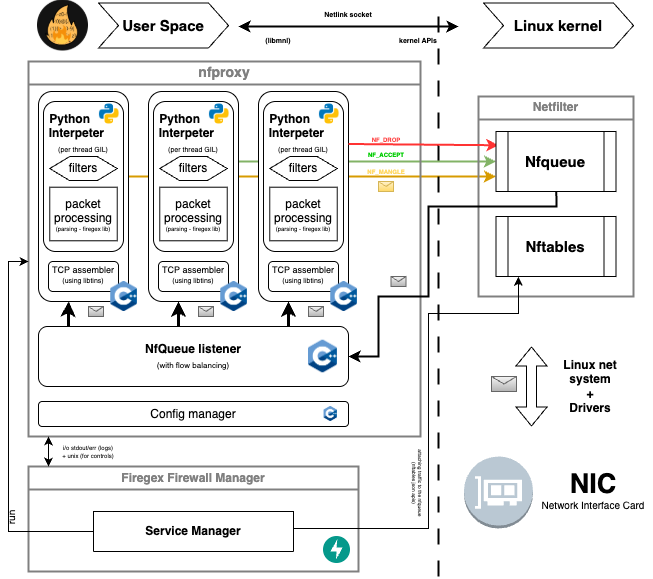
\includegraphics[width=0.9\textwidth]{images/chapter3/nfproxy.drawio.png}
    \caption{Architettura del modulo nfqueue}
    \label{fig:firegex_nfproxy_arch}
\end{figure}

\section{Elaborazione parallelizzata dei pacchetti}

Uno dei principali ostacoli affrontati durante la progettazione è stata proprio la gestione della parallelizzazione dei processi di elaborazione, 
a causa di una serie di problematiche descritte in seguito riguardo il funzionamento di \texttt{nfqueue}, alcune caratteristiche il linguaggio
python, e anche la necessità di far interfacciare 2 linguaggi differenti in un unico modulo.\\
Obiettivi principali della paralellizzazione sono stati:
\begin{itemize}
    \setlength{\itemsep}{5pt}
    \setlength{\parskip}{5pt}
    \item \texttt{Evitare la possibilità di conflitti di dati tra i processi}: Elemento critico nella progettazione per cui si devono evitare quanto possibile i conflitti
    tra i vari processi di modo da evitare corruzione di dati, crash improvvisi e comportamenti inaspettati.
    \item \texttt{Evitare l'utilizzo di elementi bloccanti quali le lock}: i lock spesso ricorrono utili nella gestione di risorse condivise, ma possono portare a problemi
    di prestazioni e di deadlock: pertanto uno degli obiettivi fissati è ridurre il loro utilizzo al minimo indispensabile, strutturando il sistema appositamente per eviatre 
    casistiche in cui è necessario il loro utilizzo.
    \item \texttt{Evitare copie in memoria, e avvio di processi sovrabbondanti}: Evitando le copie in memoria dei pacchetti, riduciamo il
    consumo di memoria ma soprattutto velociziamo il processo di analisi garantendo maggiori performance.
\end{itemize}
Per le motivazioni sopra citate, si è scelto un approccio alla parallelizzazione di tipo produttore-consumatore, che vede come produttore
un processo ascoltatore, che riceve dal kernel i pacchetti da elaborare, il quale fa effettivamente il binding della \texttt{nfqueue},
e diversi processi consumatori che hanno come uniche risorse comuni delle dequeue di pacchetti, che verranno distribuiti dal produttore.
Il produttore quindi accoderà i pacchetti in queste code, che verranno prevelati dai relativi consumatori per essere elaborati.
Il singolo consumatore si occupa di ordinare i pacchetti TCP, elaborare i filtri python, ed infine mandare i
\texttt{verdicts}\footcite{\url{https://netfilter.org/projects/libnetfilter_queue/doxygen/html/group__nfq__verd.html}}{vedicts_nfqueue}
al kernel per eseguire l'azione richiesta sul pacchetto, e procedere con la prossima elaborazione.\\
Per ogni consumatore ci sarà una coda di pacchetti separata condivisa unicamente con il produttore, la quale sarà l'unico elemento critico in cui verranno utilizzate le lock.\\
Si specifica che si è pensato anche ad una scelta implementativa diversa per le dequeue tramite l'utilizzo delle \texttt{unix pipe}\footcite{\url{https://man7.org/linux/man-pages/man2/pipe.2.html}}{unix_pipe},
tuttavia si è scelto di utilizzare un'implementazione che fa utilizzo di \texttt{std::mutex}\footcite{\url{https://en.cppreference.com/w/cpp/thread/mutex}}{std_mutex} e
\texttt{std::condition\_variable}\footcite{\url{https://en.cppreference.com/w/cpp/thread/condition_variable}}{condition_variable_std} per ragioni di performance
e di possibilità di implementare un sistema di blocco della coda in push in caso di riempimento che ferma il processo produttore (evitando di riempire eccessivamente queste code).
L'implementazione utilizzata è stata quella di \texttt{Arif Jaffer}\footcite{\url{https://www.bit-byter.com/blog/files/blocking-q-cpp.html}}{blocking_queue_cpp}.

\subsection{A Per-Interpreter GIL con python 3.12}

Una delle problematiche citate precedentemente sulla paralelizzazione erano riguardo una caratteristica del linguaggio python,
il \texttt{GIL}\footcite{Understanding the python gil}{beazley2010understanding} (Global Interpeter Lock), che limita l'utilizzo dei thread in python
permettendo ad un solo thread per volta l'esecuzione del codice, che altrimenti presenterebbe problemi riguardo la gestione degli oggetti python stessi
poichè internamente (come ad esempio per il sistema di reference counting) la loro gestione non è implementata in maniera thread-safe e incorrerebbe a comportamenti inaspettati.\\
Inoltre si sottlinea come python in questa casistica gestisce unicamente operazioni CPU-bound, che vanno ulteriormente ad evidenziare gli svantaggi portati dal GIL.\\

\begin{figure}[H]
    \centering
    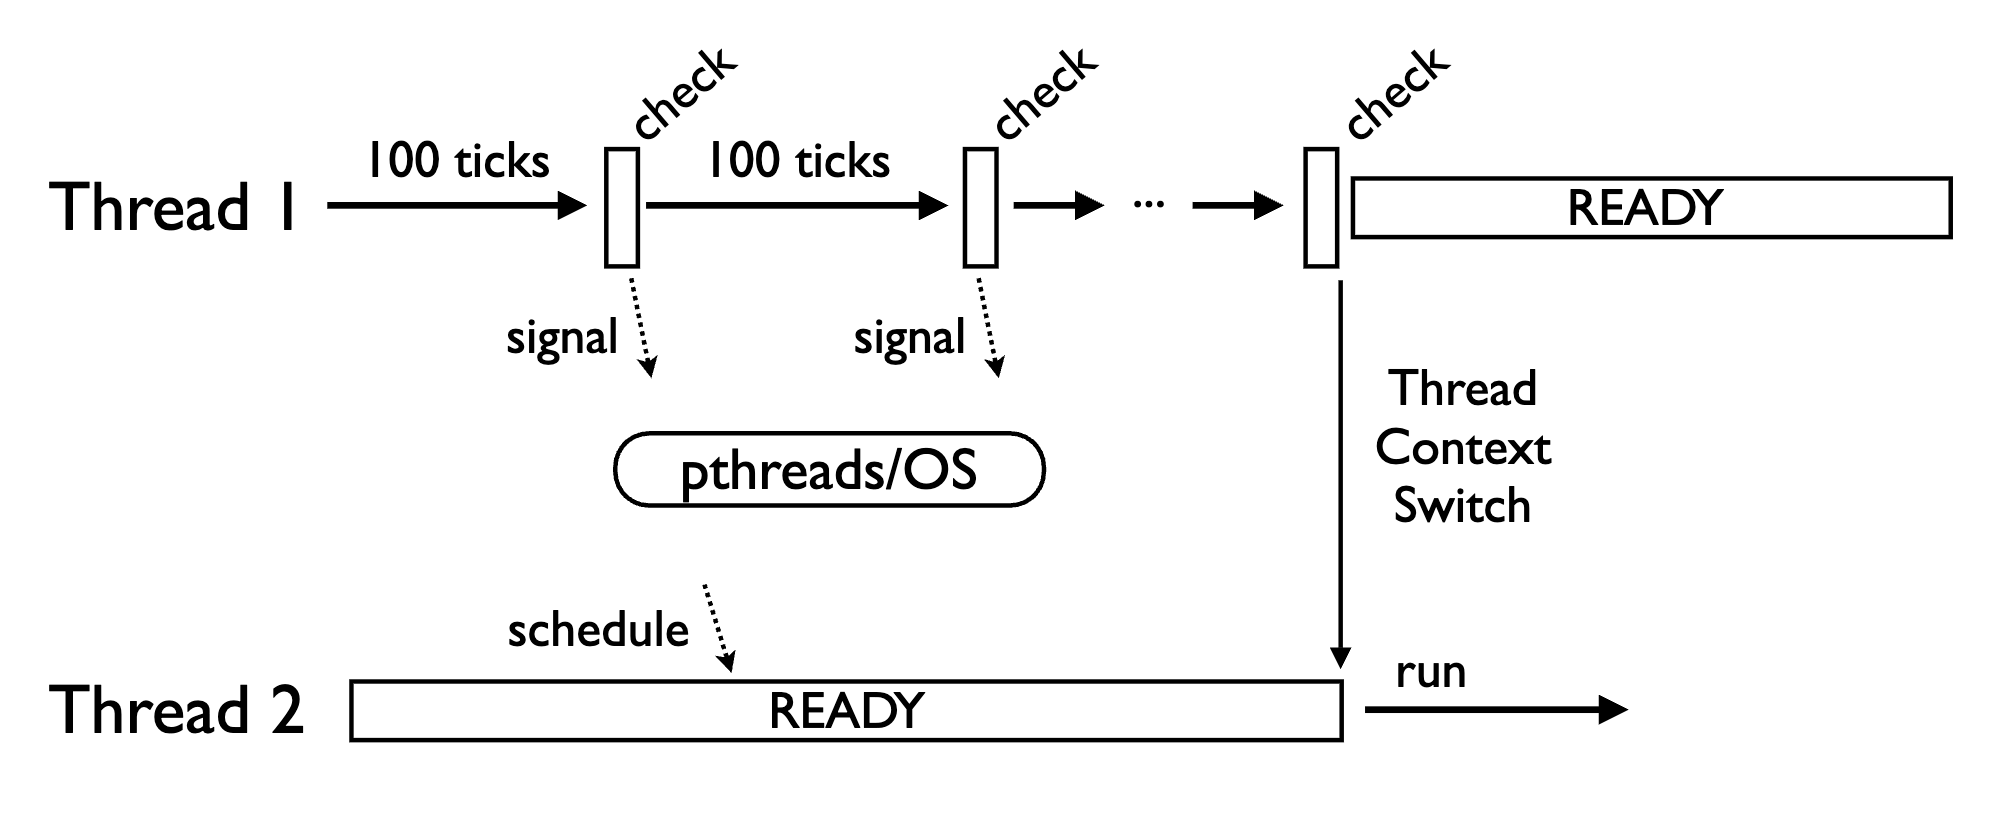
\includegraphics[width=0.8\textwidth]{images/chapter3/GIL.png}
    \caption{Python Global Interpeter Lock}
    \label{fig:py_gil_schema}
\end{figure}

Una soluzione potrebbe essere sarebbe quella di utilizzare processi multipli, che permettono di avere un GIL per ogni processo,
ma che porterebbe ad un overhead per la necessità di aggiuntivi inter-process communication con i nuovi processi, e di copia di elementi in memoria.\\

La soluzione adottata per questo problema è relativa ad una importante modifica in \texttt{Python 3.12} relativa al
\texttt{PEP 684}\footcite{\url{https://peps.python.org/pep-0684/}}{pep648}, che introduce la possibilità di avviare sullo stesso processo diversi interpreti python
ogniuno con il proprio GIL, permettendo l'esecizione di codice python in thread realmente parallelizzati.\\
L'utilizzo di questa funzionalità è unicamente accessibile tramite C-API, che ci permettono anche l'avvio diretto di un interprete python senza l'effettivo avvio dell'eseguibile
\texttt{python3}, ma direttamente tramite chiamate a \texttt{libpython}, permettendo anche alternare i 2 linguaggi facilmente.\\

Questo ha come limite il fatto che non è possibile condividere oggetti tra gli interpreti python, che però nella casistica corrente non è un problema, dato che non
ci sarà bisogno di condividere dati tra i thread, grazie al meccanismo di distribuzione dei pacchetti utilizzato descritto nel prossimo paragrafo che ne permette un completo isolamento.\\
Pertanto, una volta arrivata una nuova configurazione di filtri, alla prima nuova richiesta di elaborazione di un pacchetto, verrà ri-compilato il codice python (nel suo bytecode) e
serializzato tramite \texttt{marshal}\footcite{\url{https://docs.python.org/3/library/marshal.html}}{marshal_python} e verrà inizializzata per ogni connessione TCP
un nuovo contesto globale python che manterrà lo stato del filtro, e verrà distrutto alla fine della connessione.\\

L'implementazione di questa funzionalità tuttavia presenta i suoi limiti sul supporto di moduli python scritti con \texttt{cython}\footcite{\url{https://cython.org/}}{cython},
o in generale moduli che ad ora non sono stati tramite \texttt{multi-phase inizialization}\footcite{\url{https://peps.python.org/pep-0489/}}{pep489}, o che semplicemente hanno elementi che non sono
thread safe a loro interno. Questi moduli non possono essere utilizzati con questa implementazione, o possono portare a comportamenti inaspettati a causa di corruzioni di memoria.\\
Alcune problematiche riscontrate riguardo questo aspetto sono descritte successivamente.\\


\begin{listing}[H]
    \begin{minted}[
        frame=single,
        framerule=0.8pt,
        fontsize=\footnotesize,
        breaklines
      ]{cpp}
PyThreadState * tstate = nullptr;
PyObject* handle_packet_code = nullptr;
PyInterpreterConfig py_thread_config = {
    .use_main_obmalloc = 0,
    .allow_fork = 0,
    .allow_exec = 0,
    .allow_threads = 0,
    .allow_daemon_threads = 0,
    .check_multi_interp_extensions = 1,
    .gil = PyInterpreterConfig_OWN_GIL,
};

void before_loop() { // Function called on thread start
    PyStatus pystatus;
    // Creating a new thread state
    tstate = PyThreadState_New(PyInterpreterState_Main());
    // Acquire the GIL and switching with a new GIL
    PyEval_AcquireThread(tstate); 
    pystatus = Py_NewInterpreterFromConfig(&tstate, &py_thread_config);
    handle_packet_code = unmarshal_code(...); //Unmarshaling compiled code
    ...
}
\end{minted}
\end{listing}

Si evidenzia come una possibile soluzione alternativa a questa potrebbe essere stata utilizzare la versione priva di GIL di
\texttt{Python 3.13 free-threaded mode}\footcite{\url{https://docs.python.org/3/whatsnew/3.13.html\#whatsnew313-free-threaded-cpython}}{py13_free_threaded},
che tuttavia è stata rilasciata come feature sperimentale non consigliata per l'utilizzo in produzione, e per altro con un calo netto di performance a causa
del mancato supporto ad alcuni sistemi di ottimizzazione.

\subsection{Bilanciamento del carico}

Per il bilanciamento del carico sui processi consumatori che eseguiranno i filtri, al fine di isolare questi processi e garantire un'equa distribuzione
dei pacchetti, si è scelto di utilizzare un meccanismo basato su hashing su IP e porta sorgente e destinazione, che ne permettono un calcolo semplice e rapido
da eseguire e allo stesso tempo garantisce che gli stessi flussi di pacchetti vengano sempre elaborati dallo stesso processo consumatore, evitando quindi che
i vari consumatori debbano condividere risorse legate ai dati salvati riguardo quel specifico flusso.\\

\begin{listing}[H]
    \begin{minted}[
        frame=single,
        framerule=0.8pt,
        fontsize=\footnotesize,
        breaklines
      ]{cpp}
// Hash function for stream_id, valid for both IPv4 and IPv6
uint32_t hash_stream_id(const stream_id &sid) {
    uint32_t addr_hash = 0;
    addr_hash ^= min_addr[0] ^ min_addr[1] ^ min_addr[2] ^ min_addr[3];
    addr_hash ^= max_addr[0] ^ max_addr[1] ^ max_addr[2] ^ max_addr[3];
    uint32_t ports = (static_cast<uint32_t>(sid.min_address_port) << 16) | sid.max_address_port;
    uint32_t hash = addr_hash ^ ports;
    hash *= 0x9e3779b9; // More randomness (multiplication with a prime)
    return hash;
}

// Banacing function for the consumers (simplified)
void __real_handler(PktRequest<Worker>* pkt) {
    // Calculate the index of the consumer
    const size_t idx = hash_stream_id(pkt->sid) % pkt->ctx->size();
    // Put the packet in the queue
    converted_pkt->ctx->queue.put(converted_pkt);
}
\end{minted}
\end{listing}

Si sottolinea come una tecnica simile sia anche utilizzata direttamente kernel space per il bilanciamento del carico dei pacchetti.
La seguente gestione è stata fatta userspace e lasciata a nfqueue kernel space (come in una precedente implementazione usata per nfregex),
poichè l'hashing eseguito nel kernel per motivi tecnici legati alla generalizzazione del modulo per protocolli diversi da quelli di cui
si è interessati per lo sviluppo di nfproxy, nell'hashing eseguito lato kernel non viene utilizzata la porta.

\begin{listing}[H]
    \begin{minted}[
        frame=single,
        framerule=0.8pt,
        fontsize=\footnotesize,
        breaklines
      ]{cpp}
static inline u32
nfqueue_hash(const struct sk_buff *skb, u16 queue, u16 queues_total, u8 family,
	     u32 initval)
{
	switch (family) {
	case NFPROTO_IPV4:
		queue += reciprocal_scale(hash_v4(ip_hdr(skb), initval),
					  queues_total);
		break;
	case NFPROTO_IPV6:
		queue += reciprocal_scale(hash_v6(ipv6_hdr(skb), initval),
					  queues_total);
		break;
	case NFPROTO_BRIDGE:
		queue += reciprocal_scale(hash_bridge(skb, initval),
					  queues_total);
		break;
	}

	return queue;
}
\end{minted}
\end{listing}

Il codice precedentemente citato viene estrapolato direttamente dal kernel linux, e 
viene utilizzato nel bilanciamento di carico dei pacchetti\footnote{\url{https://web.git.kernel.org/pub/scm/linux/kernel/git/torvalds/linux.git/tree/net/netfilter/xt_NFQUEUE.c?h=v6.14-rc7\#n86}},
e il codice utilizzato per l'hashing\footnote{\url{https://web.git.kernel.org/pub/scm/linux/kernel/git/torvalds/linux.git/tree/include/net/netfilter/nf_queue.h?h=v6.14-rc7\#n105}}
come è possibile vedere non include la porta, che è stata aggiunta per il bilanciamento del carico in userspace.\\

Questo rappresenta un limite importante per l'utilizzo di questo modulo in contesti come le competizioni Attack Defence dove
troviamo traffico anonimizzato tramito l'ausilio di un NAT, che di per se pertanto porterebbe
ad un bilanciamento del carico non esistente poichè 1 solo consumatore verrebbe impegnato nell'elaborazione di tutti i pacchetti
se 1 solo ip è utilizzato nel NAT.\\
Di seguito si riporta un benchmark del modulo \texttt{nfregex} che utilizza il nuovo sistema di bilanciamento del carico userspace,
che simula del carico in elaborazione del traffico con il seguente codice:

\begin{listing}[H]
    \begin{minted}[
        frame=single,
        framerule=0.8pt,
        fontsize=\footnotesize,
        breaklines
      ]{cpp}
volatile int x = 0;
for (int i=0; i<50000; i++){
    x+=1;
}
\end{minted}
\end{listing}

\begin{figure}[H]
    \centering
    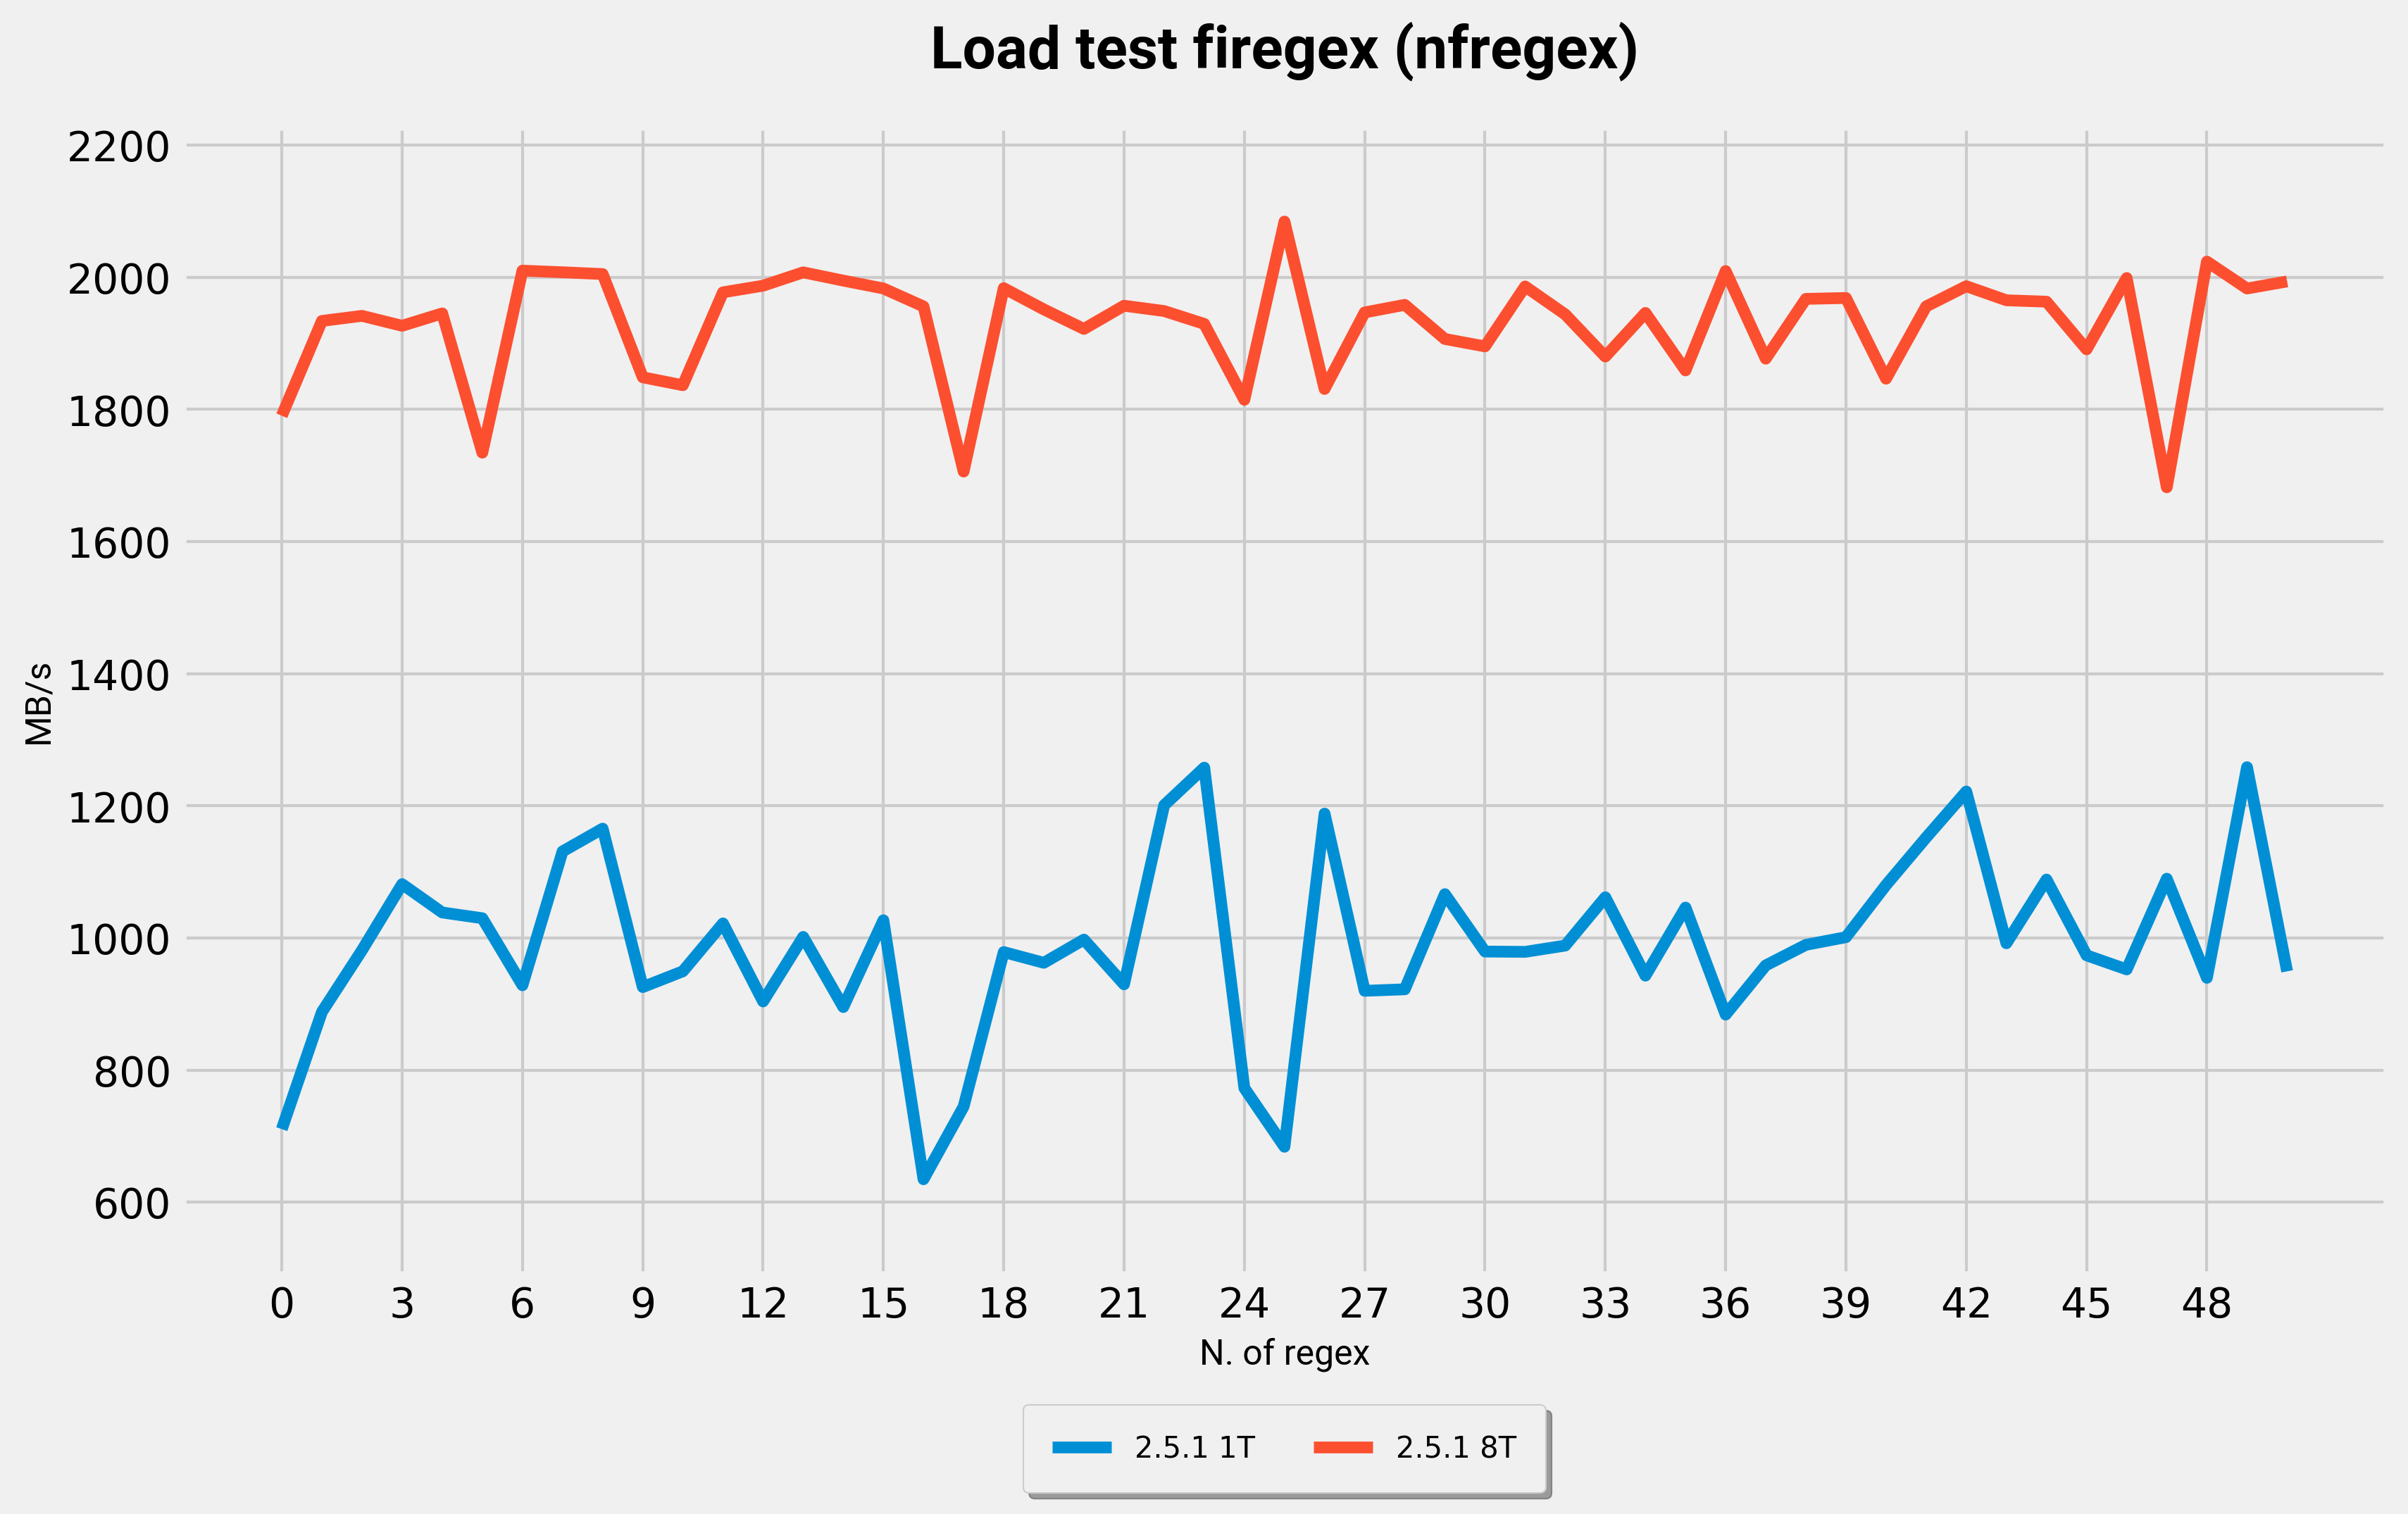
\includegraphics[width=0.98\textwidth]{images/chapter3/Benchmark-chart-with-load.png}
    \caption{NfProxy Benchmarks con load balancing personalizzato con 1 e 8 thread}
    \label{fig:nfproxy_multithread_benchmark}
\end{figure}

Gli stessi benefici sono presenti in nfproxy, infatti la base di codice per il bilanciamento dei pacchetti e la medesima per entrambi i moduli.

\section{Parsing dei pacchetti L3}

Arrivati i pacchetti nella nfqueue, questi vengono immediatamente analizzati per determinare il protocollo di livello 3,
che viene manualmente verificato tramite l'analisi dei primi 4 bit che rappresentano sia in IPv4 e in IPv6 il campo \texttt{version}.
Una volta determinata la versione del protocollo, il pacchetti viene passato ai parser per i relativi protocolli di \texttt{libtins}\footcite{\url{https://libtins.github.io/}}{libtins}.
Libtins ricorsivamente analizza i layer successivi, e ci permette di calcolare in maniera automatica lo \texttt{stream\_id},
un tipo di dato implementato nella libreria in grado di rappresentare univocamente una connessione tarmite ip e porta sorgente e destinazione in maniera ordinata:
l'ordinamento avviene prendendo la tupla ip:porta relavtivi allo stesso host come un unico valore, ed è poi l'intera tupla che veine ordinata
(se avessimo ordinato ip e porta non considerandoli a coppie, avremmo un identificativo che potrebbe essere facilmente soggetto a conflitti e per fino soggetto a
possibili attacchi al fine di bypassare i filtri del firewall stesso).
L' ordinamento permette di mantenere lo stesso identificativo sia per i pacchetti in ingresso che per i pacchetti in uscita, e dell'utilizzo di questo
dato in strutture dati come le \texttt{map}\footcite{\url{https://en.cppreference.com/w/cpp/container/map}}{std_map} utilizzate per memorizzare gli stati dei flussi.\\

\begin{listing}[H]
    \begin{minted}[
        frame=single,
        framerule=0.8pt,
        fontsize=\footnotesize,
        breaklines
      ]{cpp}
//Costruttore di PktRequest: classe che rappresenta un pacchetto effettivamente scambiata tra produttori e consumatori
PktRequest(const char* payload, size_t plen, T* ctx, mnl_socket* nl, nfgenmsg *nfg, nfqnl_msg_packet_hdr *ph, bool is_input):
    ctx(ctx), nl(nl), res_id(nfg->res_id),
    packet_id(ph->packet_id), is_input(is_input),
    packet(string(payload, plen)),
    action(FilterAction::NOACTION),
    is_ipv6((payload[0] & 0xf0) == 0x60) //Controllo della versione del protocollo
{
    if (is_ipv6){
        ipv6 = new Tins::IPv6((uint8_t*)packet.c_str(), plen); //Parsing IPv6
        sid = stream_id::make_identifier(*ipv6); // calcolo stream_id
        _original_size = ipv6->size();
    }else{
        ipv4 = new Tins::IP((uint8_t*)packet.c_str(), plen); //Parsing IPv4
        sid = stream_id::make_identifier(*ipv4); // calcolo stream_id
        _original_size = ipv4->size();
    }
    l4_proto = fill_l4_info(); // Analisi del layer di trasporto
}
\end{minted}
\end{listing}

Inoltre questo tipo di dato è agnostico rispetto al protocollo di livello 3, e pertanto può essere usato anche per un traffico misto IPv4 e IPv6, che attualmente
non è previsto per le regole e il funzionamento imposto nella fase di "inserimento" della queue nella coda di traffico, poichè ne verifichiamo che il protocollo
sia lo stesso, ma che sarebbe possibile tramite le tables L3 agnostiche di nftables, o anche semplicemente intercettando il traffico tramite diverse regole alla stessa queue,
o perfino se intercettato tramite il nome di un'interfaccia di rete che gestisce diversi indirizzzi IP, anche di versioni L3 differenti.\\
Avendo memoria condivisa, nel passaggio tra produttore e consumatore, l'analisi del pacchetto non viene persa, poichè nel passaggio del pacchetto, viene rilasciato l'indirizzo
di memoria all'oggetto c++ che rappresenta il pacchetto, la responsabilità di deallocare questa area di memoria passa al consumatore che quindi non dovrà
analizzare nuovamente il pacchetto, ma potrà direttamente procedere con la sua elaborazione.

\section{Gestione dei pacchetti TCP}

Come citato precedentemete, prima di inizializzare la queue, vengono inseriti tramite nftables le regole per intercettare il traffico in un certo punto della catena
di netfilter, per essere mandato alla queue che determinerà un verdetto sul pacchetto.\\

\begin{figure}[H]
    \centering
    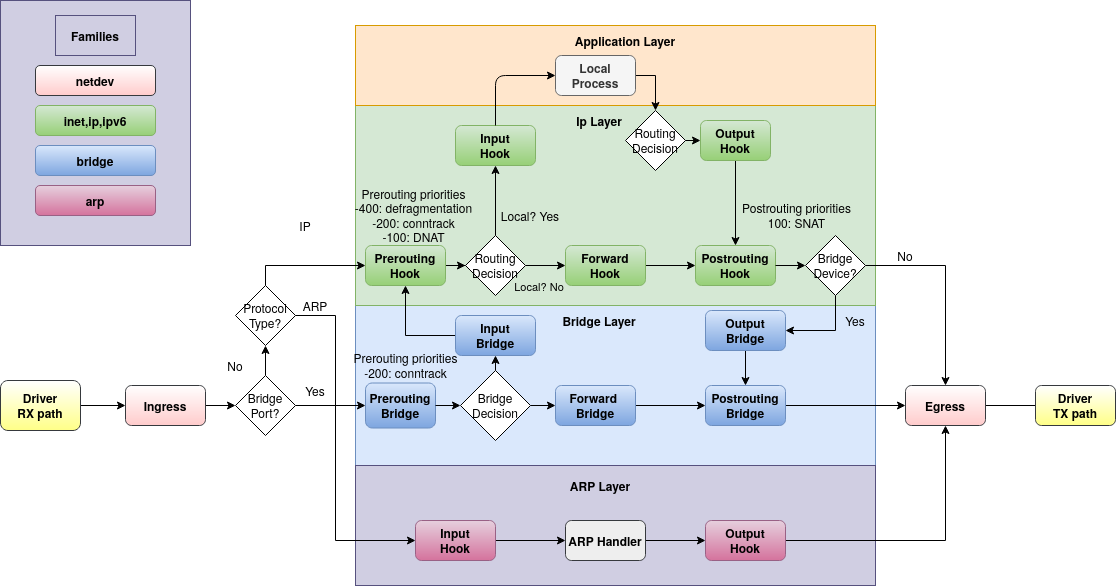
\includegraphics[width=0.98\textwidth]{images/chapter3/nf-hooks.png}
    \caption{NfTables Hooks}
    \label{fig:nftables_hooks}
\end{figure}

Il traffico in particolare viene intercettato sia in \texttt{pre-routing}, che in \texttt{post-ruoting} ad un hook prima dell'azione del modulo conntrack, ma dopo
dell'azione di defrag, in particolare a prio -310 che rientra in questo range come riportato sulla \texttt{wiki ufficiale di nftables}\footcite{\url{https://wiki.nftables.org/wiki-nftables/index.php/Netfilter_hooks}}{netfilter_hooks}.
Questo permette di ottenere dei pacchetti che hanno già subito il processo di deframmentazione a livello 3, di cui pertanto non ci dovremo preoccupare,
che non hanno subito il processo di routing (che quindi volendo potremmo manipolare) e che non sono stati ancora analizzati dal modulo conntrack.\\
Tuttavia i pacchetti non hanno subito il processo di ordinamento dei payload che avviene a livello 4, sul quale come è possibile osservare dalla figura \ref{fig:nftables_hooks}, non è possibile
intercettare del traffico, poichè i pacchetti arriveranno direttamente alle fasi di gestioni dei dati per la loro consegna alla socket a livello applicatvo.\\
Pertanto è dato a noi il compito di analizzare il traffico e di ordinare i pacchetti TCP per un'analisi dei dati coerente con ciò che sarà letto
dall'applicazione.\\
Fortunatamente, libtins ci permette di fare ciò in maniera automatica, e ha una gestione sufficientemente efficiente sullo scadere dei flussi TCP, sulla gestione dei buffer
e sulle problematiche di segmenti non ordinto dei pacchetti, che solleva l'applicativo da un numero importante di problematiche che andrebbero gestiste
manualmente, ma che ci vengono già gestiste nell'analisi stessa dei flussi TCP\footnote{Esempio TCP Follower: \url{https://libtins.github.io/examples/http-requests/}}.\\
Oltre al contesto creato all'interno dell'oggetto follower di libtins, viene creato uno stato esternamente per lo stesso flusso, per la memorizzatione
dello stato del flusso memorizzato con python, deallocato e allocato in maniera coerente al follower stesso, che tramite delle callback ci permette di
richiamare le azioni da eseguire sui dati che allochiamo.\\
Da notare che avremo un follower per ogni processo consumatore che analizzerà una sotto parte dei flussi dell'intero traffico, l'hashing ci garantisce che
lo stesso flusso verrà analizzato dallo stesso processo consumatore.
Anche il TCP follower è agnostico rispetto al protocollo di livello 3, e pertanto può essere utilizzato anch'esso per un traffico misto IPv4 e IPv6.

\section{Modifica dei pacchetti}

Il modulo nfqueue permette la modifica dei pacchetti, e pertanto la possibilità sia di modificare gli header ip e tcp, che il payload del livello di trasporto.
La modifica dei pacchetti seppur non essenziale è parzialmente supportata, ma non pienamente funzionante: questo a causa di diverse problematiche che nascono
dalla modifiche dei pacchetti stessi per diversi meccaniscmi applicati a livello di trasporto, e alucne di queste problematiche non sono di fatto
risolte a causa della loro complessità implementativa e a diverse conseguenze che potrebbero portare ad ulteriori problematiche ancora più complesse e tendenzalmente target di possibili attacchi.
Pertanto i rischi che l'applicazione di queste modifiche potrebbero sono sufficientemente elevati da non essere ritenuti tollerabili rispetto alle reali esigenze di questa funzionalità (tendenzalmente nulle).\\

Le problematiche sul calcolo dei campi di integrità dei dati sono date come risolte tramite l'utilizzo di libtins, che si occupa nella serializzazione del pacchetto e
anche di ricalcolare questi campi nei vari layer interessati, e pertanto non sono state considerate problematiche rilevanti.\\

L'unica operazione aggiuntiva affrontata su questa problematica è stata la necessità di reinserire il payload del pacchetto nella catena di PDU di libtins,
poichè (seppur non documentato), il follower del flusso TCP internamente separa di fatto il payload dal pacchetto, e pertanto è necessario reinserirlo per una
corretta serializzazione del pacchetto modificato.\footnote{Separazione del payload nel follower: \url{https://github.com/mfontanini/libtins/blob/b7e61f4c76ac64053c9c4c9f8eadaabbe3a9381a/src/tcp_ip/data_tracker.cpp\#L68}}.\\

Di seguito si riporta una descrizione accurata delle problematiche riscontrate e delle soluzioni proposte, o applicate con relativi limiti e valutazione di rischio/beneficio.\\

\subsection{Cambio di dimensione del payload}

Come emerge dalle specifiche stesse del protocollo di trasporto TCP\footcite{RFC9293, Transmission Control Protocol (TCP)}{rfc9293}, il protocollo tiene traccia
dello stato della corretta recezione dei pacchetti tramite un meccanismo di \texttt{piggybacking} che fa utilizzo dei campi numerici ack e seq.
Nella trasmissione il sequence number indica il byte da cui inizia il payload del pacchetto relativamente alla sua posizione nello stream, mentre nel campo ack della risposta
di conferma proveniente dal ricevente, viene indicato fino a che punto il flusso di dati è stato ricevuto ordinato e corretto.\\
Questo meccanismo è fondamentale per il corretto funzionamento del protocollo e per la ricostruzione del flusso originale,
e di conseguenza una modifica sulla dimensione del payload causa una conseguente incoerenza di questi valori che portano comportamenti inaspettati e non conformi rispetto al 
normale funzionamento del protocollo.\\

Per risolvere questa problematica, si è implementato un sistema di conversione dei campi ack e seq, che permette una conversione di questi valori tale da
mantenere la corretta sequenza di numeri in uscita che conferma al client che il pacchetto ricevuto è stato correttamente ricevuto per qual'era la sua grandezza originale,
e il kernel (ma anche il follower di libtins stesso) di aver avuto un riscontro su un pacchetto che sia della dimensione del pacchetto ricevuta sulla base della modifica effettuata.
Lo stesso meccanismo ma applicato in maniera opposta viene applicato per i dati e che arrivano a loro volta dalla direzione opposta.\\
Si noti come dalla prima modifica di un pacchetto, il sistema di conversione viene attivato, e viene mantenuto attivo e funzionante per tutta la connessione, per
mantenere coerenti i numeri di ack e seq.\\

La conversione degli ack e seq avviene tramite il calcolo incrementale dell'offset che intercorre tra la dimensione del flusso originale e la dimensione del flusso modificato,
calcolata come si può osservare nel seguente codice:

\begin{listing}[H]
    \begin{minted}[
        frame=single,
        framerule=0.8pt,
        fontsize=\footnotesize,
        breaklines
      ]{cpp}
size_t payload_offset = data_size() != _data_original_size;
// If we are in a TCP connection, the ack and seq status context was enabled, and the payload size 
if (tcp && ack_seq_offset && payload_offset != 0){
    // So we incrementally update the total offset based on how sent this data.
    if (is_input){
        ack_seq_offset->in += payload_offset;
    }else{
        ack_seq_offset->out += payload_offset;
    }
}
\end{minted}
\end{listing}

A seguito della modifica, nei prossimi pacchetti vengono compatibilmente ricalcolati gli ack e seq, su tutto il traffico come si può vedere nel seguente codice:

\begin{listing}[H]
    \begin{minted}[
        frame=single,
        framerule=0.8pt,
        fontsize=\footnotesize,
        breaklines
      ]{cpp}
void fix_tcp_ack(){
    // Checks if the conversion is needed
    need_tcp_fixing = need_tcp_fix();
    if(!need_tcp_fixing){
        return;
    }
    // Convertion of the ack and seq
    if (is_input){
        tcp->seq(tcp->seq() + ack_seq_offset->in);
        tcp->ack_seq(tcp->ack_seq() - ack_seq_offset->out);
    }else{
        tcp->ack_seq(tcp->ack_seq() - ack_seq_offset->in);
        tcp->seq(tcp->seq() + ack_seq_offset->out);
    }
}
\end{minted}
\end{listing}

Da un'analisi superficiale, e da dei semplici test sembrerebbe che la soluzione sia sufficiente alla risoluzione del seguente problema, tuttavia la seguente logica
non riesce a risolvere tutte le problematiche che possono sorgere dalla modifica della dimensione del payload:\\
di fatto questo meccanismo è funzionale solo nel caso in cui non vi siano problemi di trasmissione, e che quindi non si presentino ritrasmissioni di pacchetti persi.\\

Il calcolo eseguito infatti non tiene in considerazione il fatto che in caso di ritrasmissione di segmenti precedenti al pacchetto modificato, il calcolo
del'ack relativo al segmento ritrasmesso deve essere eseguito risfasarlo come dovrebbe essere fatto per i pacchetti successivi, mentre l'implementazione
attuale esegue questa conversione non valutando quale sia la parte del flusso che si sta effettivamente riscontrando.\\

\begin{figure}[H]
    \centering
    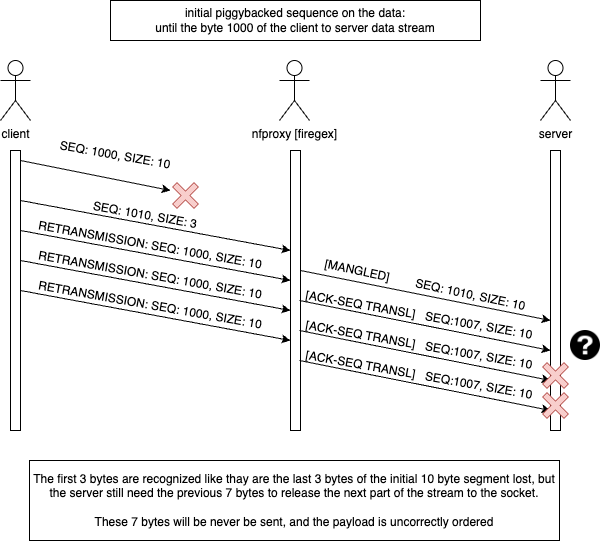
\includegraphics[width=0.98\textwidth]{images/chapter3/TCP_ack_seq_transl_failure.drawio.png}
    \caption{Esempio di una possibile problematica nella traduzione di ack e seq implementata}
    \label{fig:tcp_ack_seq_transl_failure}
\end{figure}

È facile comprendere osservando la figura \ref{fig:tcp_ack_seq_transl_failure} come queste casistiche possano far completamente
decadere il sistema di traduzione implementato, che potrebbero essere frequenti in casi di congestione del traffico e diventare
un elemento di interesse per eventuali attacchi miratamente incentrati su questo tipo di problematica (che tuttavia porterebbero ad una
interruzione del normale andamento del traffico, e quindi non ne consegue in un effettivo vantaggio da parte dell'attaccante nello scenario di nostro interesse).\\

Concludiamo pertanto che la soluzione proposta non è sufficientemente robusta per essere considerata una soluzione definitiva, e pertanto la modifica dei pacchetti viene si
offerta come possibilità, ma segnalata come funzionalità instabile che potrebbe portare a comportamenti inaspettati.\\

Una possibile soluzione robusta dovrebbe prevedere la memorizzazione del punto in cui il flusso è stato effettivamente modificato congiuntamente con l'offset utilizato fino
a quel punto in quella direzione del traffico, finchè i dati fino a quegli intervalli non viene riscontrato dal ricevente e non solo:
dovrebbe prevedere una logica che risulta particolarmente complessa per la traduzione di ack e seq, poichè deve tenere conto di tutta una serie di possibili scenari
come il caso di frequenti modifiche di pacchetti in sucecssione con ritrasmissioni, ma anche i casi di ri-trasmissioni di pacchetti con payload composti da dati
che precedentemente erano stati inviati in pacchetti differenti.\\
Andando a trattare tutte le casistiche l'implementazione diventa via via sempre più complessa da realizzare, per cui si ritene poco utile
il suo effettivo sviluppo dato la risicata utilità della funzionalità stessa.

\subsection{Modifica di segmenti non ordinati}

Un ulteriorie problema nasce dalla necessità di modificare i pacchetti con dei payload out-of-order da modificare:
nella attuale implementazione in caso arrivino dei paccheti non ordinati, questi vengono analizzati dal TCP follower di libtins, che considera il payload per
la ricostruzione del flusso, ma successivamente il pacchetto viene automaticamente accettato, e pertanto non si avrà la possibilità di modificarlo in seguito.\\
In caso quel pacchetto conteneva un payload malevolo, ad esso verrà comunque impedito di passare a livello applicativo, poichè nel momento in cui arriverà
il pacchetto contenete il payload che completerebbe il flusso disordinato, questo verrà analizzato dal filtro insieme al payload precedete (supponendo ce ne sia solo 1),
e bloccato: pertanto il flusso ricostruito dal kernel non verrà mai ricostruito completamente e la connessione degenererà in una chiusura forzata.\\

Tuttavia se vogliamo avere completo controllo sulla modifica del traffico la seguente soluzione non è praticabile: una possibile alternativa richiederebbe
di non accettare i pacchetti out-of-order, e di memorizzare i pacchetti in un buffer fino a che non arrivi il pacchetto mancante, e di procedere con la modifica
di diversi pacchetti riportando le modifiche effettuate sul flusso ricostruito distribuendolo nei segmenti trattenuti nella queue.\\
La seguente soluzione tuttavia richiederebbe la gestione di un importante livello di complessità a livello di ricostruzione delle modfiche, ma soprattutto
porterebbe alla considerazione una nuova categorie di problematiche legate al riempimento della nfqueue lato kernel, che potrebbe facilmente essere soggetta
ad un riempimento e quindi alla conseguente perdita dei pacchetti successivi. Se i pacchetti in coda per essere elaborati necessitano dell'analisi di pacchetti che nel
frattempo verranno scartati dalla nfqueue, ci troveremo in una situazione di stallo in cui si verificherebbe il blocco totale del traffico.\\
La seguente logica può essere implementata da un attaccante che con un'adeguata costruzione di traffico malevolo può molto facilmente
sfruttare questa problematica per eseguire un attacco \texttt{DoS} di rilevante importanza.\\
Per le considerazioni fatte, si può comprendere come sia di fondamentale importanza che i pacchetti elaborati abbiano un riscontro immediato che non
debba dipendere da altri pacchetti, garantendo quindi il continuo fluire del traffico nella coda lato kernel.\\

Per queste casistiche sono stati pensati diversi meccanismi che permetterebbero di mitigare il problema, ma nessuno di questi rimane
sufficientemente robusto da essere resiliente a possibili attacchi attacchi DoS, e pertanto si è deciso di escludere la possibilità
di accodare i pacchetti facendoli rimanere in attesa di ulteriori pacchetti: \texttt{il loro riscontro al modulo nfqueue deve essere immediatamente al termine dell'elaborazione}
come avviene nell'implementazione attuale.\\

\section{Parsing dei pacchetti HTTP}

A seguito di una ricerca riguardo soluzioni già esistenti per il parsing dei pacchetti HTTP, non ho trovato soluzioni che fossero adeguate
alle richieste del progetto, sopratutto data la necessaria compatibilità dei moduli le funzionalità introdotte nel
\texttt{PEP 684}\footcite{\url{https://peps.python.org/pep-0684/}}{pep648} che come precedentemente, richiedono l'implementazione di moduli
con \texttt{multi-phase inizialization}\footcite{\url{https://peps.python.org/pep-0489/}}{pep489} e che siano thread safe.\\
Pertanto partendo dall'implementazione trovata online di \texttt{Derrick Lyndon Pallas}\footcite{Python wrapper per llhttp: \url{https://github.com/pallas/pyllhttp}}{original_pyllhttp_impl},
basata sul modulo \texttt{llhttp}\footcite{\url{https://github.com/nodejs/llhttp}}{llhttp} utilizzato nell'interprete di \texttt{Node.js}, ho deciso di
sviluppare un fork di questo modulo, con alcuni fix e con il supporto al \texttt{PEP 684} disponibile
su github\footcite{\url{https://github.com/domysh/pyllhttp}}{pyllhttp_fork} e su \texttt{pypi}\footnote{\texttt{https://pypi.org/project/pyllhttp/}}
per consentirne l'installazione e l'utilizzo tramite \texttt{pip}. La versione HTTP compatibile è la 1.1.

\subsection{Supporto agli algoritmi di compressione HTTP}

Nel traffico HTTP sono spesso in uso algoritmi di compressione per ridurre la dimensione del body,
compatibilmente con quanto descritto nell'\texttt{RFC 2616}\footcite{RFC2616, Hypertext Transfer Protocol -- HTTP/1.1}{rfc2616}.

Dato il suo ampio utilizzo, al fine di semplificare l'implementazione di filtri che necessitano di analizzare il body dei pacchetti HTTP,
si è deciso di implementare il supporto agli algoritmi di compressione supportati da browser chrome:

\begin{itemize}
    \setlength{\itemsep}{5pt}
    \setlength{\parskip}{5pt}
    \item \texttt{gzip}\footcite{RFC1952, GZIP file format specification version 4.3}{rfc1952}: Nativamente supportato in python.
    \item \texttt{brotli}\footcite{RFC7932, Brotli Compressed Data Format}{rfc7932}: Il seguente algoritmo di compressione è supportato tramite
    un'implementazione e il relativo wrapper python sviluppato da \texttt{google} che tuttavia non supporta il \texttt{PEP 684}, e per cui ho sviluppato
    il fork compatibile con le specifiche del progetto disponibile su github\footcite{\url{https://github.com/domysh/brotli}}{brotli_fork}.
    \item \texttt{zstd}\footcite{RFC8478, Zstandard Compression and the application/zstd Media Type}{rfc8478}: Algoritmo di compressione sviluppato da \texttt{Meta},
    che non ha sviluppato direttamente un wrapper python, che tuttavia è stato sviluppato da \texttt{Sergey Dryabzhinsky}\footcite{\url{https://github.com/sergey-dryabzhinsky/python-zstd}}{zstd_ortiginal_python_wrapper},
    anch'esso però non compatibile con il \texttt{PEP 684}, e per cui ho sviluppato un fork compatibile disponibile su github\footcite{\url{https://github.com/domysh/python-zstd}}{zstd_fork}.
    \item \texttt{deflate}\footcite{RFC1951, DEFLATE Compressed Data Format Specification version 1.3}{rfc1951}: Implementabile tramite il modulo \texttt{zlib}.
\end{itemize}

L'implementazione è stata scritta seguendo le specifiche definite nell'\texttt{RFC 2616} il quale definisce la possibilità di compressioni multiple, correttamente
supportate nell'implementazione finale.
    
\subsection{Supporto alle websocket}

Nel supporto ad HTTP/1.1 è stato incluso anche il supporto alle \texttt{websocket}\footcite{RFC6455, The WebSocket Protocol}{rfc6455},
con l'utilizzo della principale libreria python utilizzata per le decodifica dei Frame websocket, ovvero \texttt{websockets}\footcite{\url{https://websockets.readthedocs.io/en/stable/}}{python_websockets}.
Del precedente modulo sono state utilizzate le funzionalità di decodifica dei frame e le funzionalità per il supporto all'estensione \texttt{permessage-deflate}\footcite{RFC7692, Compression Extensions for WebSocket}{rfc7692},
per permettere la decompressione dei frame compressi (che utilizza la libreria \texttt{zlib}, resa già compatibile al supporto per il \texttt{PEP 684}).
La complessità nell'implementazione delle websocket si è concentrata sulla necessità di assemblare il flusso di dati correttamente per permettere
la decodifica dei Frame che normalmente non supporta uno streaming parsing come nel caso di \texttt{llhttp}, e nella fase di upgrading della connessione per il
riconoscimento dei plugin abilitati nella specifica connessione websocket.\\
In caso di fallimento nel parsing dei frame, i dati vengono resi disponibili al filtraggio come dati TCP ordinati (la stessa cosa succede in caso di upgrade ad HTTP/2).

\section{Sintassi e gestione dei filtri python}

I filtri python deiniti per nfproxy devono essere scritti in un singolo file (per servizio) che può contenere una serie di funzioni chiamate
\texttt{pyfilters} che possono richiedere determinati dati, e possono restituire degli \texttt{statment} che definiscono il comportamento da eseguire elaborato
al termine dell'elaborazione eseguita.\\

Di seguito un esempio di un filtro python che blocca i pacchetti provenienti da un client che utilizza il browser \texttt{curl} e che
richiede un upgrade a websocket:

\begin{listing}[H]
    \begin{minted}[
        frame=single,
        framerule=0.8pt,
        fontsize=\footnotesize,
        breaklines
      ]{python}
from firegex.nfproxy.models import HttpRequest
from firegex.nfproxy import pyfilter
from firegex.nfproxy import REJECT

@pyfilter
def curl_filter(r: HttpRequest):
    if r.upgrading_to_ws:
        return REJECT # Reject the request if request is upgrading to websocket
    if "curl" in r.user_agent:
        print(f"Tried to access with curl: {r.user_agent}")
        return REJECT # Reject the request if user agent is curl
\end{minted}
\end{listing}

Come si può notare il filtro utilizza la libreria \texttt{firegex}, pubblicata su \texttt{pypi}\footcite{\url{https://pypi.org/project/firegex/}}{firegex_pypi},
da cui è possibile importare il decorator utilizzato per definire i filtri, e le classi utilizzate per la definizione dei dati che vengono passati.\\

NfProxy infatti analizza in fase di compilazione le signature delle funzioni definite come filtri, eseguendo in automatico il codice per
eseguire il parsing dei dati richiesti e chiama le funzioni, passando come argomenti i dati richiesti.\\
Pertanto i pyfilters prendono il nome della funzione stessa, e supportano un numero variabile di parametri che tuttavia devono necessariamente
avere un tipo definito in \texttt{firegex.nfproxy.models} come decorator, necessario a comprendere la struttura dei dati che necessita di essere passata,
sullo stesso principio utilizzato da \texttt{pydantic}\footcite{\url{https://docs.pydantic.dev/latest/}}{pydantic}, nota libreria python.\\

Le funzioni possono restituire uno \texttt{statment} che definisce il comportamento da eseguire, tra i principali \texttt{ACCEPT}, \texttt{REJECT} e \texttt{DROP}.
Se la funzione non restituisce nulla (o restituisce \texttt{None}), il pacchetto verrà accettato.\\

Ulteriori dettagli sull'utilizzo dei models (chiamati anche datahandler) sono disponibili nella documentazione integrata nell'interfaccia di \texttt{firegex} per nfproxy.

\subsection{Gestione dei buffer di memoria}

Il parsing dei pacchetti per traffico con una dimensione di payload elevata, può portare ad un consumo eccessivo di memoria, e pertanto è necessario
gestire in maniera efficiente i buffer di memoria utilizzati per la memorizzazione dei pacchetti.\\
Di default nfproxy utilizza un buffer di memoria di massimo 1MB per ogni tipo di datahandler utilizzato, superato il quale il buffer viene svuotato
evitanto quando possibile la rottura del parsing stesso.\\

Questo comportamento può essere modificato tramite l'utilizzo delle variabili globali di nfproxy, che permettono di modificare il comportamento
in base alle esigenze sia potendole rendere più restrittive limitando il consumo di RAM, sia potendole rendere più permissive, permettendo
di memorizzare più dati in memoria. Inoltre è anche possibile modificare il comportamento in caso di superamento del limite imposto, permettendo
di scegliere se svuotare il buffer, accettare il pacchetto, rifiutare la connessione o eseguendone il drop dei pacchetti successivi.\\

Di seguito un estratto della documentazione integrata in nfproxy che descrive le variabili globali utilizzate per la gestione dei buffer di memoria:

\begin{listing}[H]
    \begin{minted}[
        frame=single,
        framerule=0.8pt,
        fontsize=\footnotesize,
        breaklines
      ]{python}
# ADVANCED OPTIONS
# You can specify some additional options on the streaming managment
# pyproxy will automatically store all the packets (already ordered by the c++ binary):
#
# If the stream is too big, you can specify what actions to take:
# This can be done defining some variables in the global context
# - FGEX_STREAM_MAX_SIZE: The maximum size of the stream in bytes (default 1MB)
#   NOTE: the stream size is calculated and managed indipendently by the data type handling system
#   Only types required by at least 1 filter will be stored.
# - FGEX_FULL_STREAM_ACTION: The action to do when the stream is full
#   - FullStreamAction.FLUSH: Flush the stream and continue to acquire new packets (default)
#   - FullStreamAction.DROP: Drop the next stream packets - like a DROP action by filter
#   - FullStreamAction.REJECT: Reject the stream and close the connection - like a REJECT action by filter
#   - FullStreamAction.ACCEPT: Stops to call pyfilters and accept the traffic

from firege.nfproxy import FullStreamAction

# Example of a global context
FGEX_STREAM_MAX_SIZE = 4096
FGEX_FULL_STREAM_ACTION = FullStreamAction.REJECT
# This could be an ideal configuration if we expect to normally have streams with a maximum size of 4KB of traffic
\end{minted}
\end{listing}

\section{Proxy di simulazione}

Per verificare il corretto funzionamento dei filtri scritti prima della loro applicazione sul firewall, è possibile
sviluppare e testare i filtri tramite un proxy di simulazione che permette di testare i filtri in un ambiente controllato
già implementato nella libreria \texttt{firegex} che oltre ad offrire le funzionalità base per la scrittura del filtro, offre
il comando \texttt{fgex} che permette di eseguire il proxy di simulazione.\\

Ad esempio con il comando \texttt{fgex nfproxy test\_http.py 127.0.0.1 8080 --proto http} è possibile eseguire il proxy di simulazione
che permette di testare i filtri scritti in \texttt{test\_http.py} su un server locale in ascolto sulla porta 8080 (la stessa cosa sarebbe possibile inserendo come
indirizzo ad esempio quello del proprio server, e simulare un attacco sulla connessione sotto proxy, per verificare il corretto funzionamento dei filtri).\\

Il proxy di simulazione riconosce automaticamente i cambiamenti nei file di filtro, e pertanto non è necessario riavviare il proxy ad ogni modifica
dei filtri, che verranno ricaricati automaticamente ed è fortemente consigliato il suo utilizzo durante la scrittura stessa
del filtro per verificare il corretto funzionamento del filtro stesso.\\

Si specifica che il simulatore utilizza la maggior parte del codice utilizzato dal firewall reale ma ovviamente non permette di analizzare e modificare il traffico
a livello di rete o di trasporto per limiti intrinsechi al fatto che è costruito tramite un proxy TCP.

\begin{figure}[H]
    \centering
    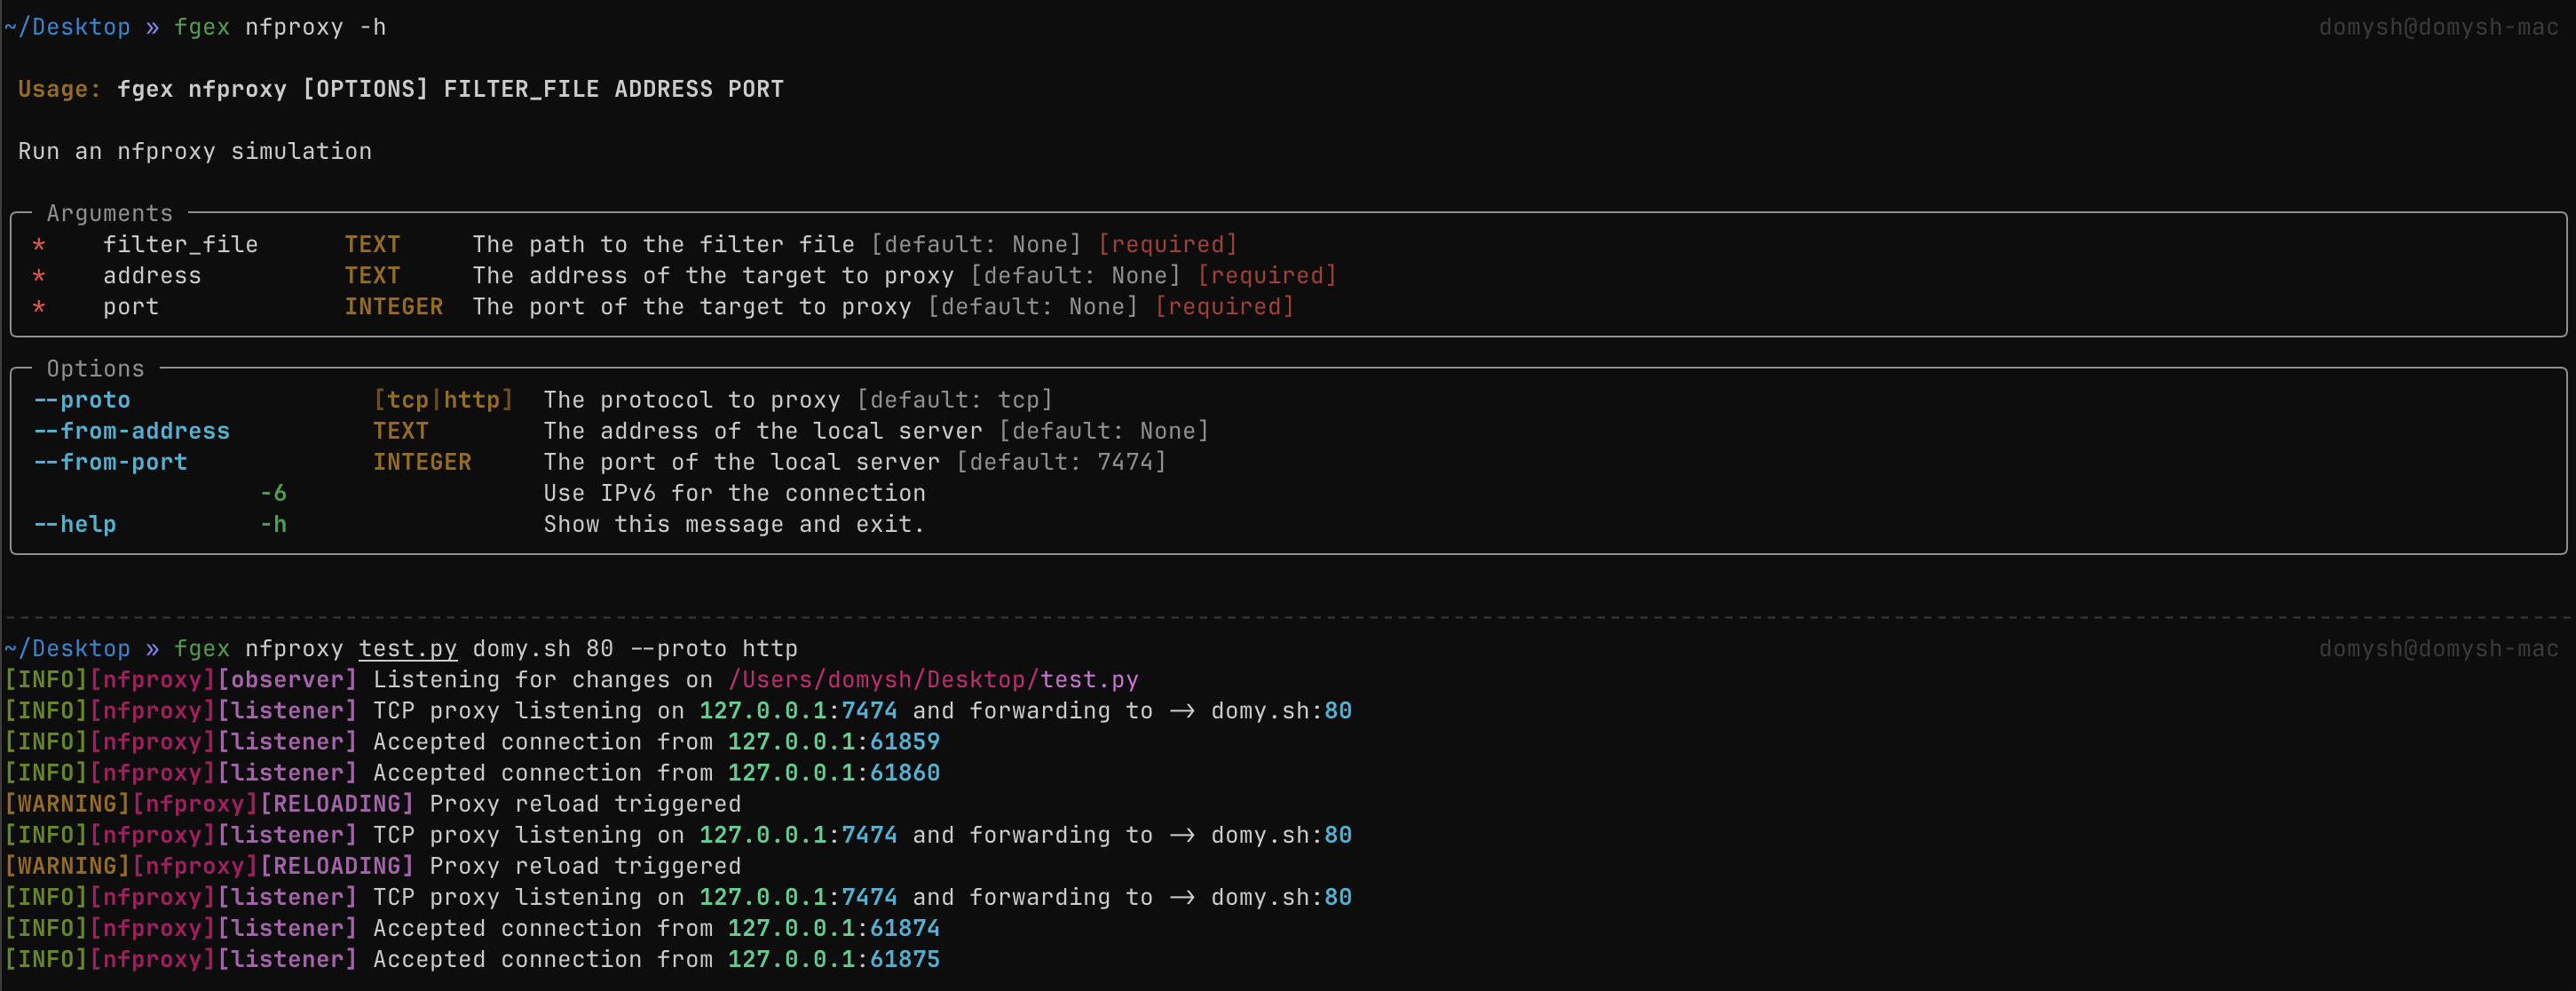
\includegraphics[width=0.98\textwidth]{images/chapter3/nfproxy_sim.png}
    \caption{Simulatore di nfproxy tramite il comando fgex}
    \label{fig:nfproxy_sim}
\end{figure}

